\documentclass[tikz, convert={density=600,outext=.png}]{standalone}
\usetikzlibrary{positioning}

\begin{document}
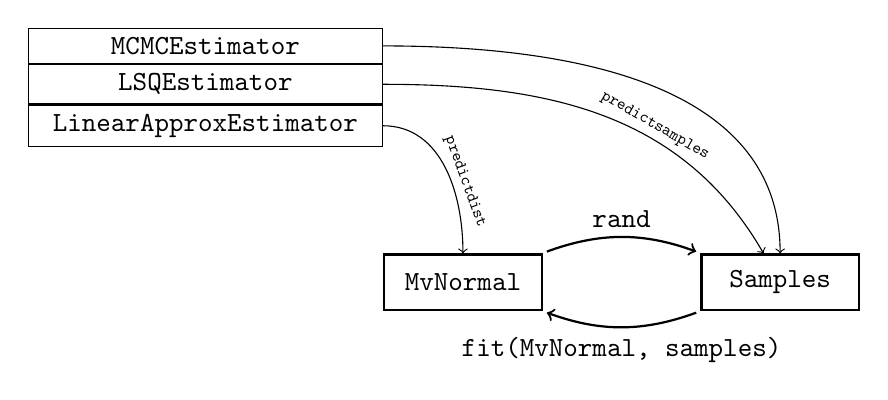
\begin{tikzpicture}[
    mybox/.style={minimum width=2.0cm, minimum height=0.70cm, draw, thick},
    myarrow/.style={shorten <=2pt, shorten >=2pt, ->, thick},
  ]
  \node[mybox] (mvnormal) {\texttt{MvNormal}};
  \node[mybox, right=2 of mvnormal, align=center] (samples) {\texttt{Samples}};

  \draw[myarrow] (mvnormal) to[bend left=20] node[above] {\texttt{rand}} (samples);
  \draw[myarrow] (samples)  to[bend left=20] node[below] {\texttt{fit(MvNormal, samples)}} (mvnormal);

  \node[draw, minimum width=4.5cm, above=3 of mvnormal.west, anchor=east] (mcmcestimator) {\texttt{MCMCEstimator}};
  \node[draw, minimum width=4.5cm, below=0 of mcmcestimator] (lsqestimator) {\texttt{LSQEstimator}};
  \node[draw, minimum width=4.5cm, below=0 of lsqestimator] (linearapproxestimator) {\texttt{LinearApproxEstimator}};
  
  \draw[->] (mcmcestimator) to[out=0, in=90] (samples);
  \draw[->] (lsqestimator) to[out=0, in=120] node[above, rotate=-30, pos=0.62, scale=0.6] {\texttt{predictsamples}} (samples);
  \draw[->] (linearapproxestimator) to[out=0, in=90] node[above, rotate=-70, scale=0.6, pos=0.62] {\texttt{predictdist}} (mvnormal);
\end{tikzpicture}
  
\end{document}
